\section*{Problem 2}

Repeat Problem 1 where $x(t) = e^{-t/4} cos(t) u(t)$

In order to examine the effects of aliasing in the time domain, plot x(t) 
for each of the sampling times for t=0 to 15 sec. 
In MATLAB, this is done by defining your time vector with the time increment set to the
desired sampling period. MATLAB then "reconstructs" the signal by 
connecting the sampled points with straight lines (this is known as a linear interpolation). 
Compare your sampled/reconstructed signals with a signal that is more accurate,
one that is created by using a very small sampling period (such as T = 0.05
sec) by plotting them on the same graph.

\subsection*{Solution}

First we calculate $X(\omega)$.
\begin{equation*}
x(t) = \frac{1}{2} \left[
	e^{-t/4}e^{jt} u(t) + e^{-t/4}e^{-jt}u(t) \right]
\end{equation*} 

Directly from (\ref{eq:c2p5}) we have:
\begin{equation*}
\begin{aligned}
X(\omega) &= \frac{1}{2} \left[
	\frac{1}{(1/4 + j) +j \omega} + 
	\frac{1}{(1/4 - j) +j \omega} \right] \\
          &= \frac{1}{2} \left[
	\frac{1}{1/4 + (\omega + 1)j} + 
	\frac{1}{1/4 + (\omega - 1)j} \right] \\
\end{aligned}
\end{equation*} 

The plot of the magintude of $X(\omega)$ is:
\zcodemat{sources/c3p21.m}{Plot of Magnitude}

\begin{figure}[H]
\caption{Magnitude $|X(\omega)|$}
\centering
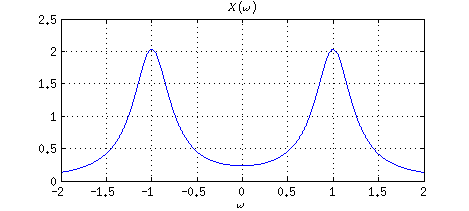
\includegraphics[width=0.8\textwidth]{figs/c3p21.png}
\label{fig:c3p21}
\end{figure} 

\begin{itemize}
\item $T_s = \pi/4 sec$
\end{itemize} 

This sampling period is lower than the minimum required and therefore no
aliasing will occur as can be seen in (\ref{fig:c3p2a}).

\begin{equation*}
\omega_s = \frac{2 \pi}{T_s} = 8 
\end{equation*} 

\zcodemat{sources/c3p2a.m}{Plot of $|X_s(\omega)|$}

\begin{figure}[H]
\caption{Sampling $|X_s(\omega)|$}
\centering
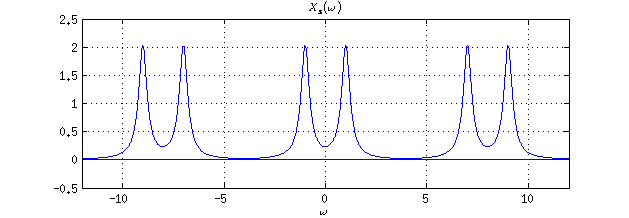
\includegraphics[width=0.6\textwidth]{figs/c3p2a.png}
\label{fig:c3p2a}
\end{figure}

\begin{itemize}
\item $T_s = \pi/2 sec$
\end{itemize} 

This sampling period is equal than the minimum required and therefore is
in the limit of no aliasing as can be seen in (\ref{fig:c3p2b}).

\begin{equation*}
\omega_s = \frac{2 \pi}{T_s} = 4
\end{equation*} 

\begin{figure}[H]
\caption{Sampling $|X_s(\omega)|$}
\centering
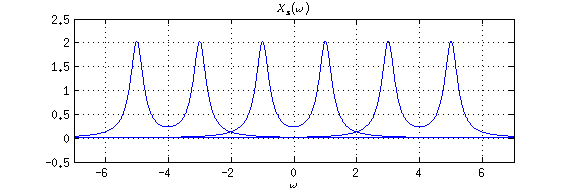
\includegraphics[width=0.6\textwidth]{figs/c3p2b.png}
\label{fig:c3p2b}
\end{figure}

\begin{itemize}
\item $T_s = 2 \pi/3 sec$
\end{itemize} 

This sampling period is lower than the minimum required and therefore 
aliasing will occur as can be seen in (\ref{fig:c3p2c}).

\begin{equation*}
\omega_s = \frac{2 \pi}{T_s} = 4
\end{equation*} 

\begin{figure}[H]
\caption{Sampling $|X_s(\omega)|$}
\centering
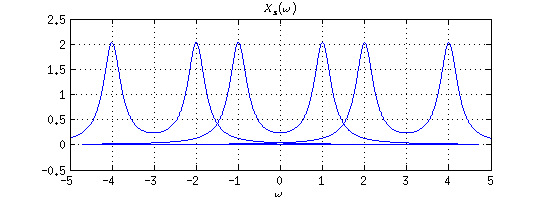
\includegraphics[width=0.6\textwidth]{figs/c3p2c.png}
\label{fig:c3p2c}
\end{figure}

Plot of "reconstructed" x(t) with MATLAB:

\zcodemat{sources/c3p2recons.m}{Plot of x(t) for different T}

\begin{figure}[H]
\caption{Reconstructed x(t)}
\centering
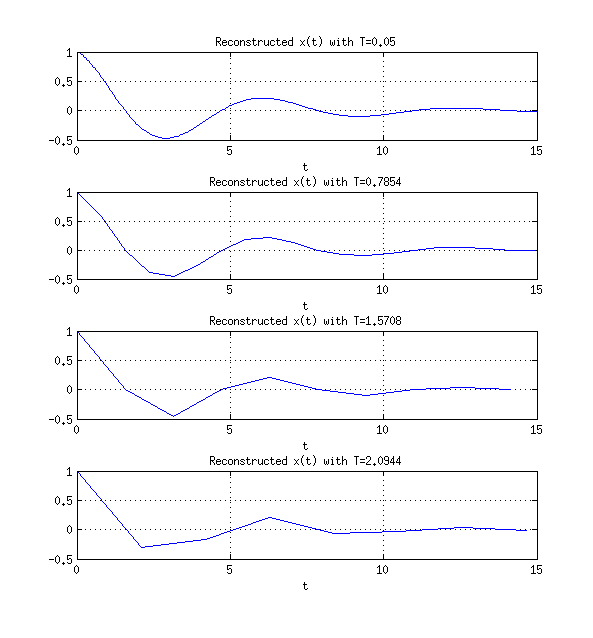
\includegraphics[width=0.8\textwidth]{figs/c3p2recons.png}
\label{fig:c3p2recons}
\end{figure} 
